\chapter{Detector Characterization}

\begin{figure}[htpb]
\centering
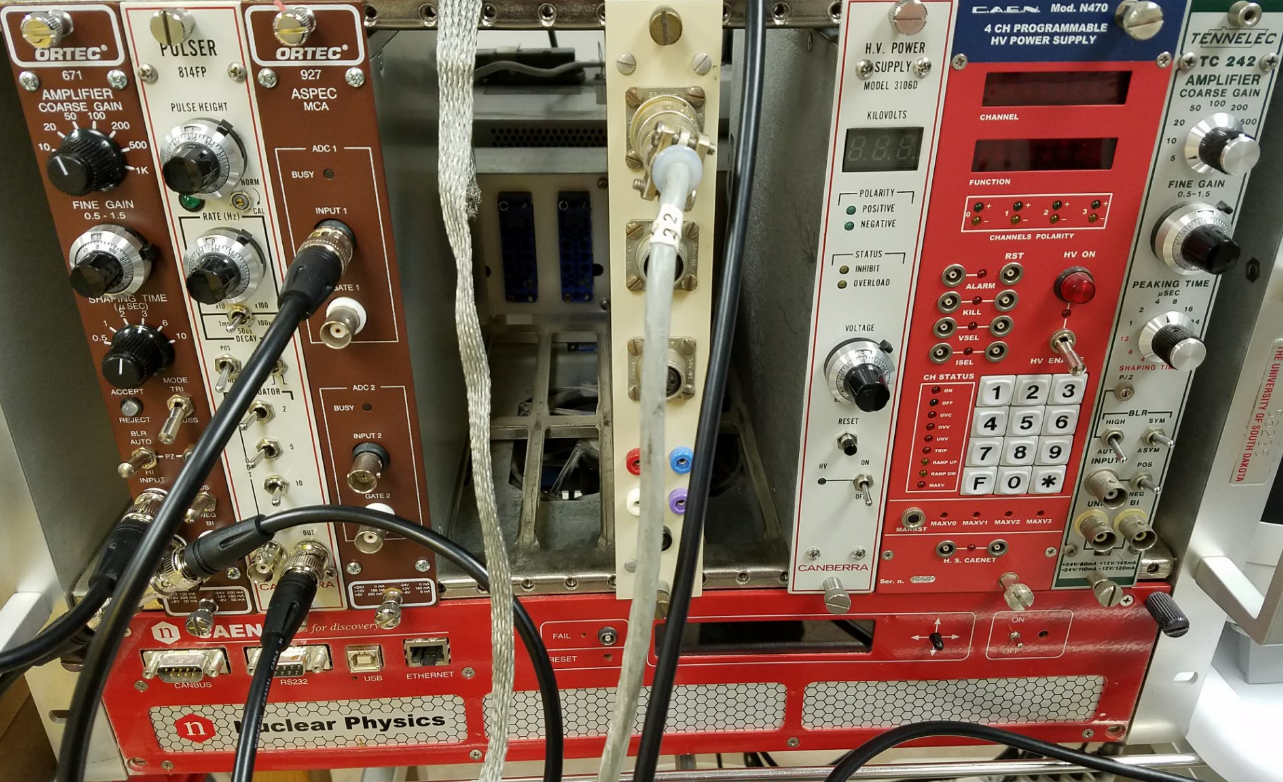
\includegraphics[width=0.7\textwidth]{crate}
\caption{Cutaway drawing of the ebeam meachanics}
\label{fig:crate}
\end{figure}

\begin{figure}[htpb]
\centering
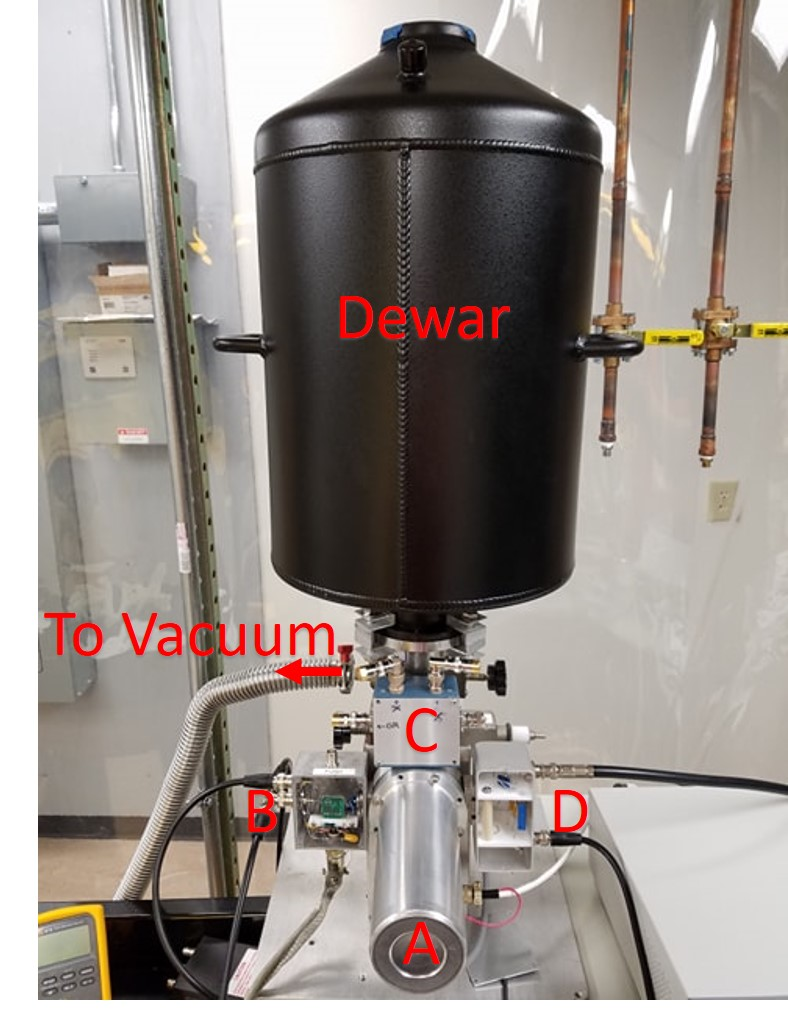
\includegraphics[width=0.7\textwidth]{cryostat-whole}
\caption{Cutaway drawing of the ebeam meachanics}
\label{fig:cryostat-whole}
\end{figure}

\begin{figure}[htpb]
\centering
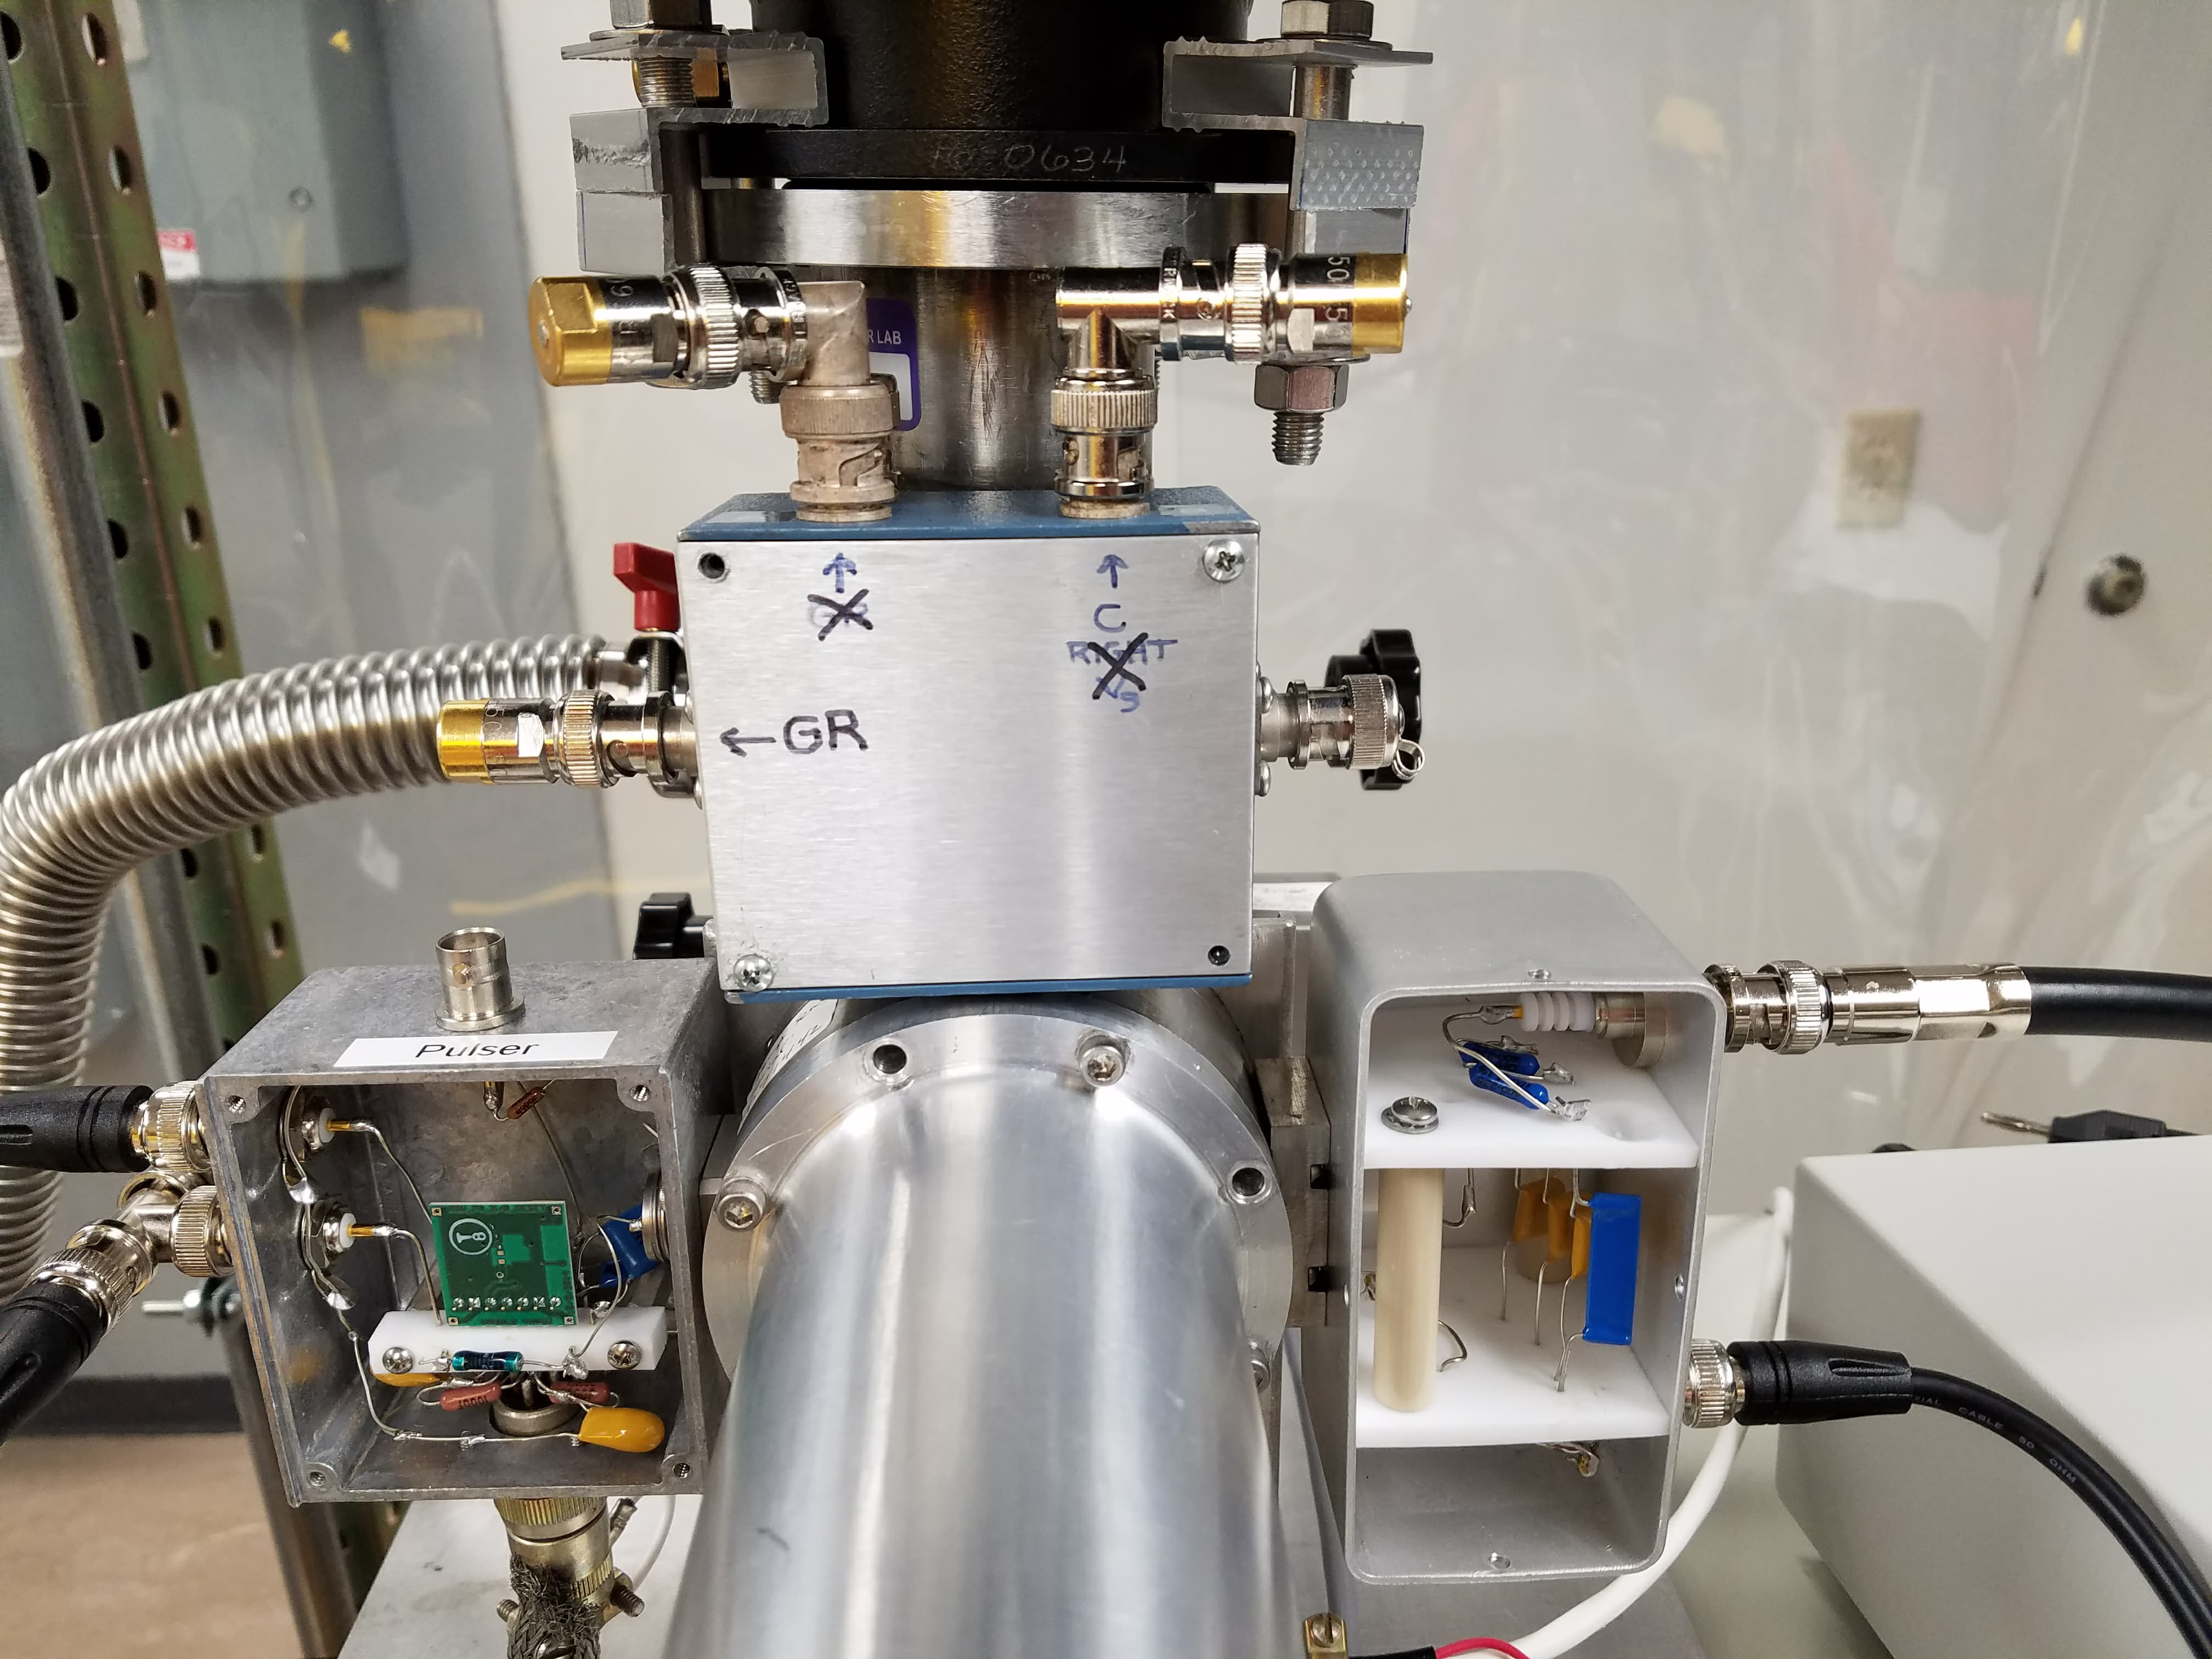
\includegraphics[width=0.7\textwidth]{inputs}
\caption{Cutaway drawing of the ebeam meachanics}
\label{fig:inputs}
\end{figure}

\begin{figure}[htpb]
\centering
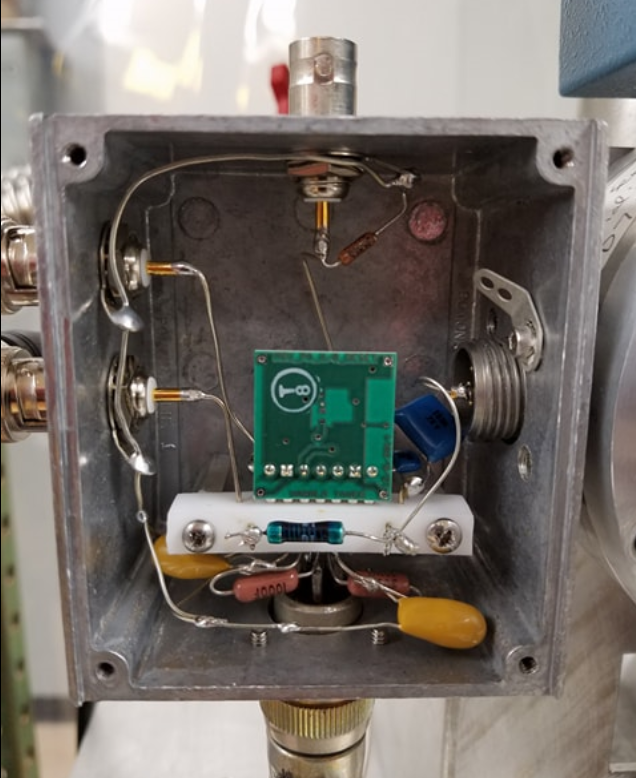
\includegraphics[width=0.7\textwidth]{left-ear}
\caption{Cutaway drawing of the ebeam meachanics}
\label{fig:left-ear}
\end{figure}

\begin{figure}[htpb]
\centering
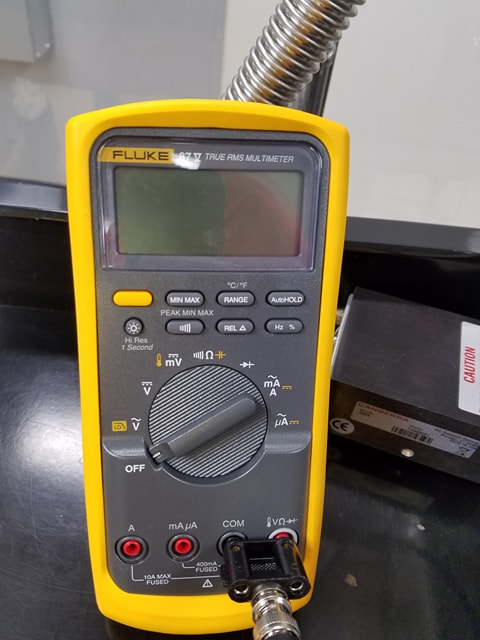
\includegraphics[width=0.7\textwidth]{multimeter}
\caption{Cutaway drawing of the ebeam meachanics}
\label{fig:multimeter}
\end{figure}

\begin{figure}[htpb]
\centering
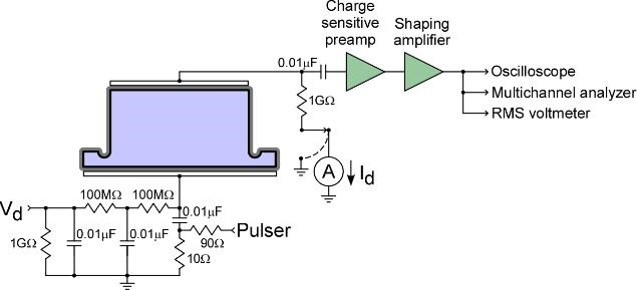
\includegraphics[width=0.7\textwidth]{outline}
\caption{Cutaway drawing of the ebeam meachanics}
\label{fig:outline}
\end{figure}

\begin{figure}[htpb]
\centering
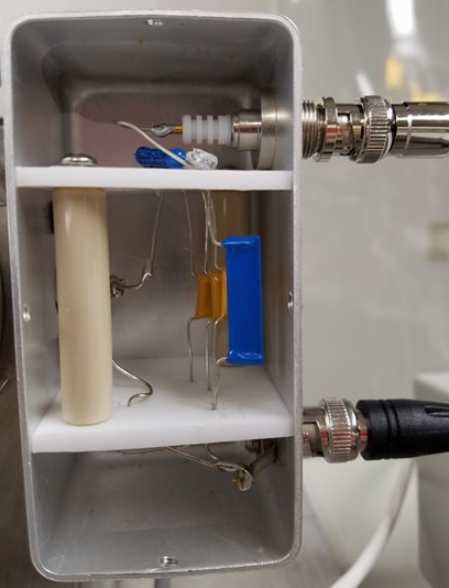
\includegraphics[width=0.7\textwidth]{right-ear}
\caption{Cutaway drawing of the ebeam meachanics}
\label{fig:right-ear}
\end{figure}

\begin{figure}[htpb]
\centering
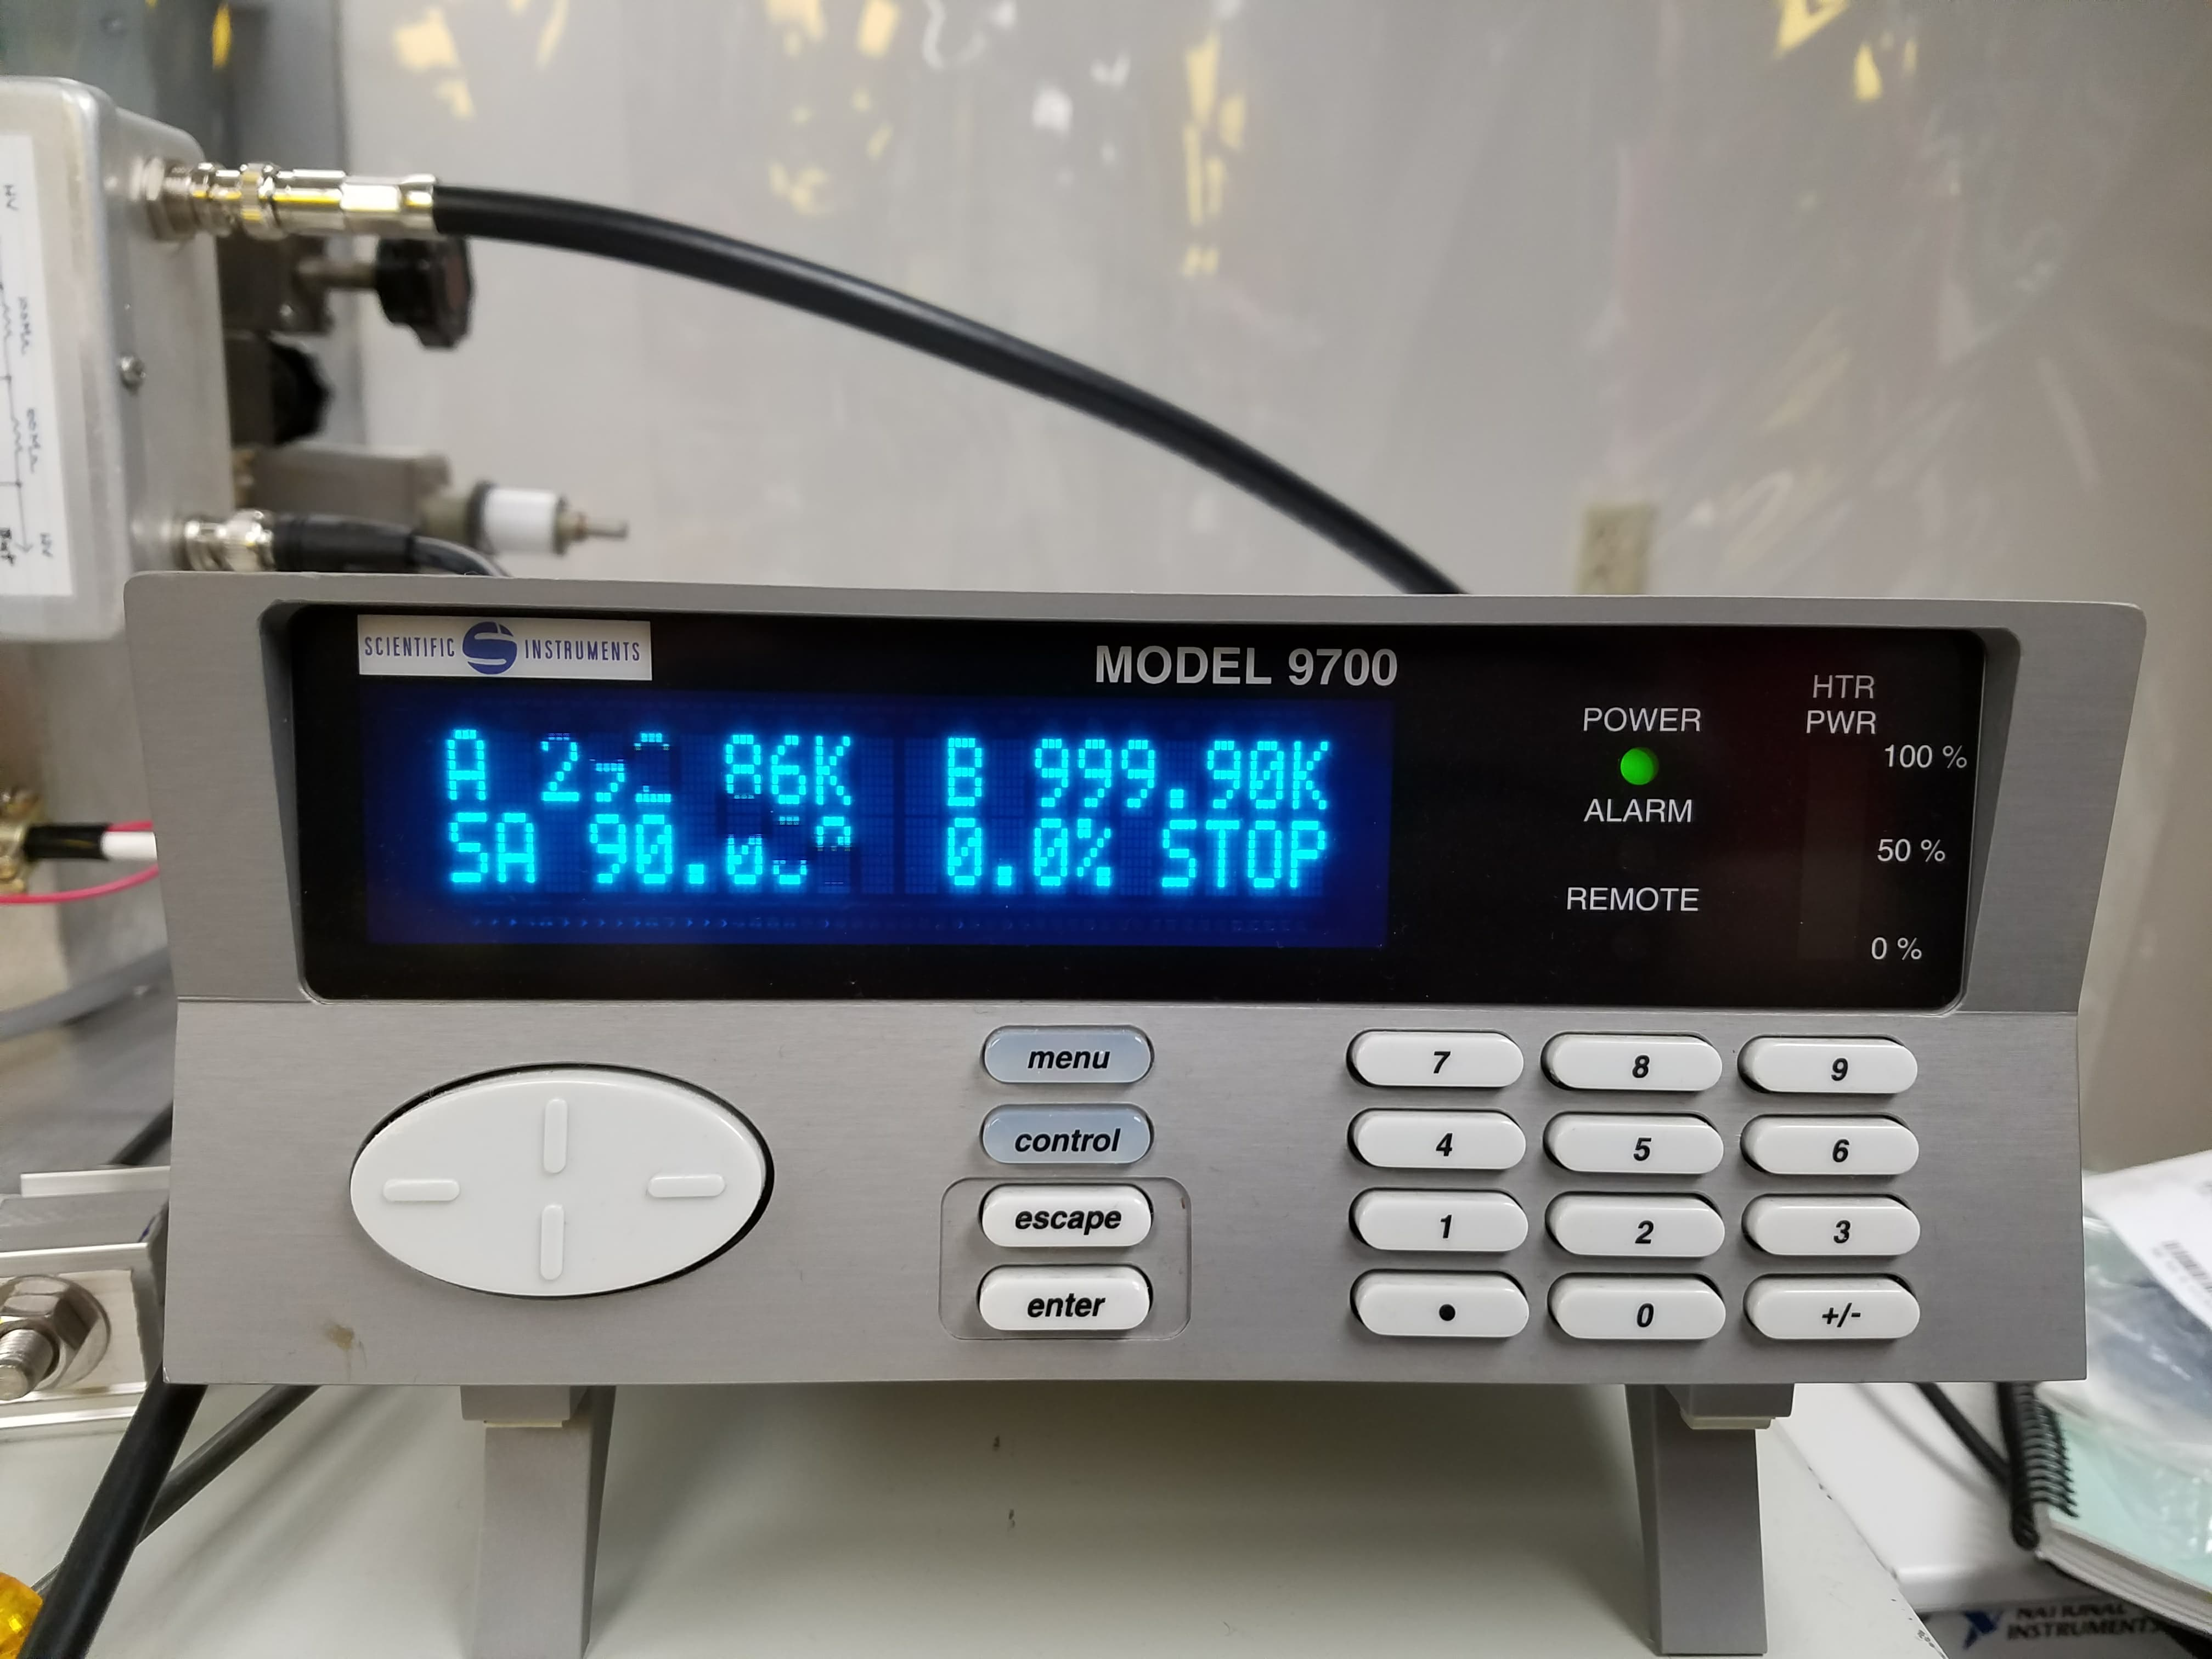
\includegraphics[width=0.7\textwidth]{temp-sens}
\caption{Cutaway drawing of the ebeam meachanics}
\label{fig:temp-sens}
\end{figure}

\begin{figure}[htpb]
\centering
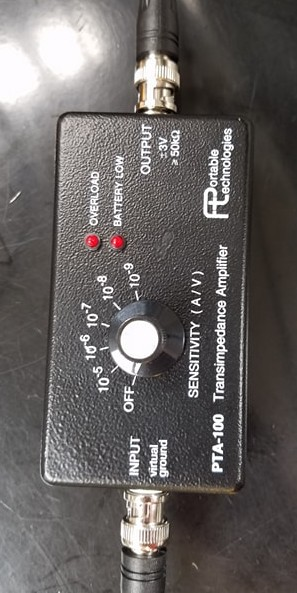
\includegraphics[width=0.7\textwidth]{transimpedence}
\caption{Cutaway drawing of the ebeam meachanics}
\label{fig:transimpedence}
\end{figure}